\documentclass[12pt,titlepage,letterpaper]{article}

\usepackage{hw}

\title{Homework I}
\author{Hanlin He (hxh160630)}
\date{\today}

\begin{document}
\maketitle

\section{IP Addressing and Subnetting}
\begin{enumerate}[label=\bfseries\alph*)]
    \item To configure B and C as a subnet, it takes at least two available IP
        address, plus the reserve address for broadcast and the subnet itself.
        So it would be a subnet with subnet mask of \texttt{30}, or in
        dot-decimal notation of \texttt{255.255.255.252}. In conclusion, the
        number of addresses available for the Ethernet would be reduced by
        four.
    \item As ARP proxy, B would pretend to be C in front of A.
        \begin{enumerate}[label=\bfseries\roman*. ]
            \item Packets send sequence would be like \cref{1ai}.
                \begin{table}[H]
                \footnotesize
                \centering
                \caption{All Packets Sent}\label{1ai}
                \begin{tabular}{c|c|c|c|c|c}
                    Message & \multirow{2}{*}{Sender} & Sender's & Sender's &
                    Target & Target \\
                    Type & & MAC Addr & IP Addr & MAC Addr & IP Addr \\\hline\hline
                    ARP Req & A & A's MAC addr & A's IP & 00-00-00-00-00-00 &
                    C's IP \\
                    ARP reply & B & B's MAC addr & C's IP & A's MAC addr &
                    A's IP \\%\hline
                    %&&&&&\\
                    IP msg & A & A's MAC addr & A's IP & B's MAC addr &
                    C's IP 
                \end{tabular}
                \end{table}
            \item To implement the proxy ARP, B's routing table need to add
                rules that for for all received or generated packets
                destination at C's IP address, the packets would go through the
                WIFI interface. And for packets received from C with
                destination address not B, B would forward the message to the
                Ethernet interface.
        \end{enumerate}
\end{enumerate}

\section{CIDR}
If the router actually containing that subset failed, the connected router
would detect that the link become unavailable and delete the ``correct''
routing policy. In the meantime, all the packets with the destination of that
subset addresses would be forwarded to the router advertising the ``big''
address blocks, since it's the only matching one, which lead to the wrong
domain.

\section{Internet Basics}
\begin{enumerate}[label=\bfseries\alph*)]
    \item The core router need to know the actual network number since the
        router still based on the routing table to forward a packet. Because
        the packet only contains a destination IP address, it does not contain
        the AS number it wants to go to. In other word, BGP only helps the
        router to build the routing table, it do not generate its own
        forwarding table.
    \item In theory, network administrator could redistribute all of the EBGP
        routes into the IGP. However, this is not recommended because of the
        large number of EBGP routes in the real Internet might cause the IGP
        crashes. By setting up iBGP among routers within an AS, and inject a
        default route (or boarder router pretend to have direct link with
        destination), the internal router could learn the best border router to
        use when sending a packet to any address.
    \item Firstly, advertising the entire AS-path would make routing loop
        easily detected. Secondly, sometimes network administrator might want
        the network traffic go through specific path due to some policy
        decisions. Only by know the entire AS-path can such requirement be
        fulfilled.
    \item Internet supports broadcast.
        Routers in Internet are able to forward broadcast messages to each LAN.
        It's LAN's duty to continue the broadcast in its network segments.
        Thus it is necessary for the LAN to be able to do a broadcast.
\end{enumerate}

\section{Routing Policies}
\begin{enumerate}[label=\bfseries\alph*)]
    \item \texttt{E} would be willing to accept advertisement from \texttt{D}
        to maximize its monetary. Since if \texttt{E} accept from \texttt{B},
        it would increase expenses. And if \texttt{E} accept from \texttt{C},
        there will be no profit, since \texttt{C} is a peer.
    \item To enforce \texttt{E} accept advertisement from \texttt{C}, network
        administrator could set up a higher local preference.
    \item \texttt{E} would prefer \texttt{A} to use AS level path
        $\mathtt{A}\rightarrow\mathtt{D}\rightarrow\mathtt{E}$. Because
        receiving traffic from \texttt{D} would increase profit via providing
        service to \texttt{D}.
    \item To cause the traffic to propagate on path 
        $\mathtt{A}\rightarrow\mathtt{D}\rightarrow\mathtt{E}$, \texttt{E} can
        prepend its AS path towards \texttt{B} and \texttt{C} to make the path
        longer. That is, instead of advertising AS path \texttt{[E]},
        \texttt{E} can advertising a longer AS path \texttt{[E,E]} to both
        \texttt{B} and \texttt{C}, and advertising the original AS path to
        \texttt{D}. By doing this, \texttt{A} would receive AS paths as:
        \begin{itemize}[label=-]
            \item \texttt{[B,E,E]} from \texttt{B},
            \item \texttt{[C,E,E]} from \texttt{C},
            \item \texttt{[D,E]} from \texttt{D}.
        \end{itemize}
        \texttt{A} would choose the shorter one,
        $\mathtt{A}\rightarrow\mathtt{D}\rightarrow\mathtt{E}$.
    \item \texttt{B}, \texttt{C} and \texttt{D} should have at least the same
        local preference at AS \texttt{A}.\\ If, otherwise, local preference of
        \texttt{D} is lower, path
        $\mathtt{A}\rightarrow\mathtt{D}\rightarrow\mathtt{E}$
        would be discarded in the first place.
\end{enumerate}

\section{Dispute Graphs}
\begin{enumerate}[label=\bfseries\alph*)]
    \item The dispute graph for the system is shown in \cref{51}.
        \begin{figure}[H]
            \centering
            \caption{Dispute Graph for Original System}\label{51}
            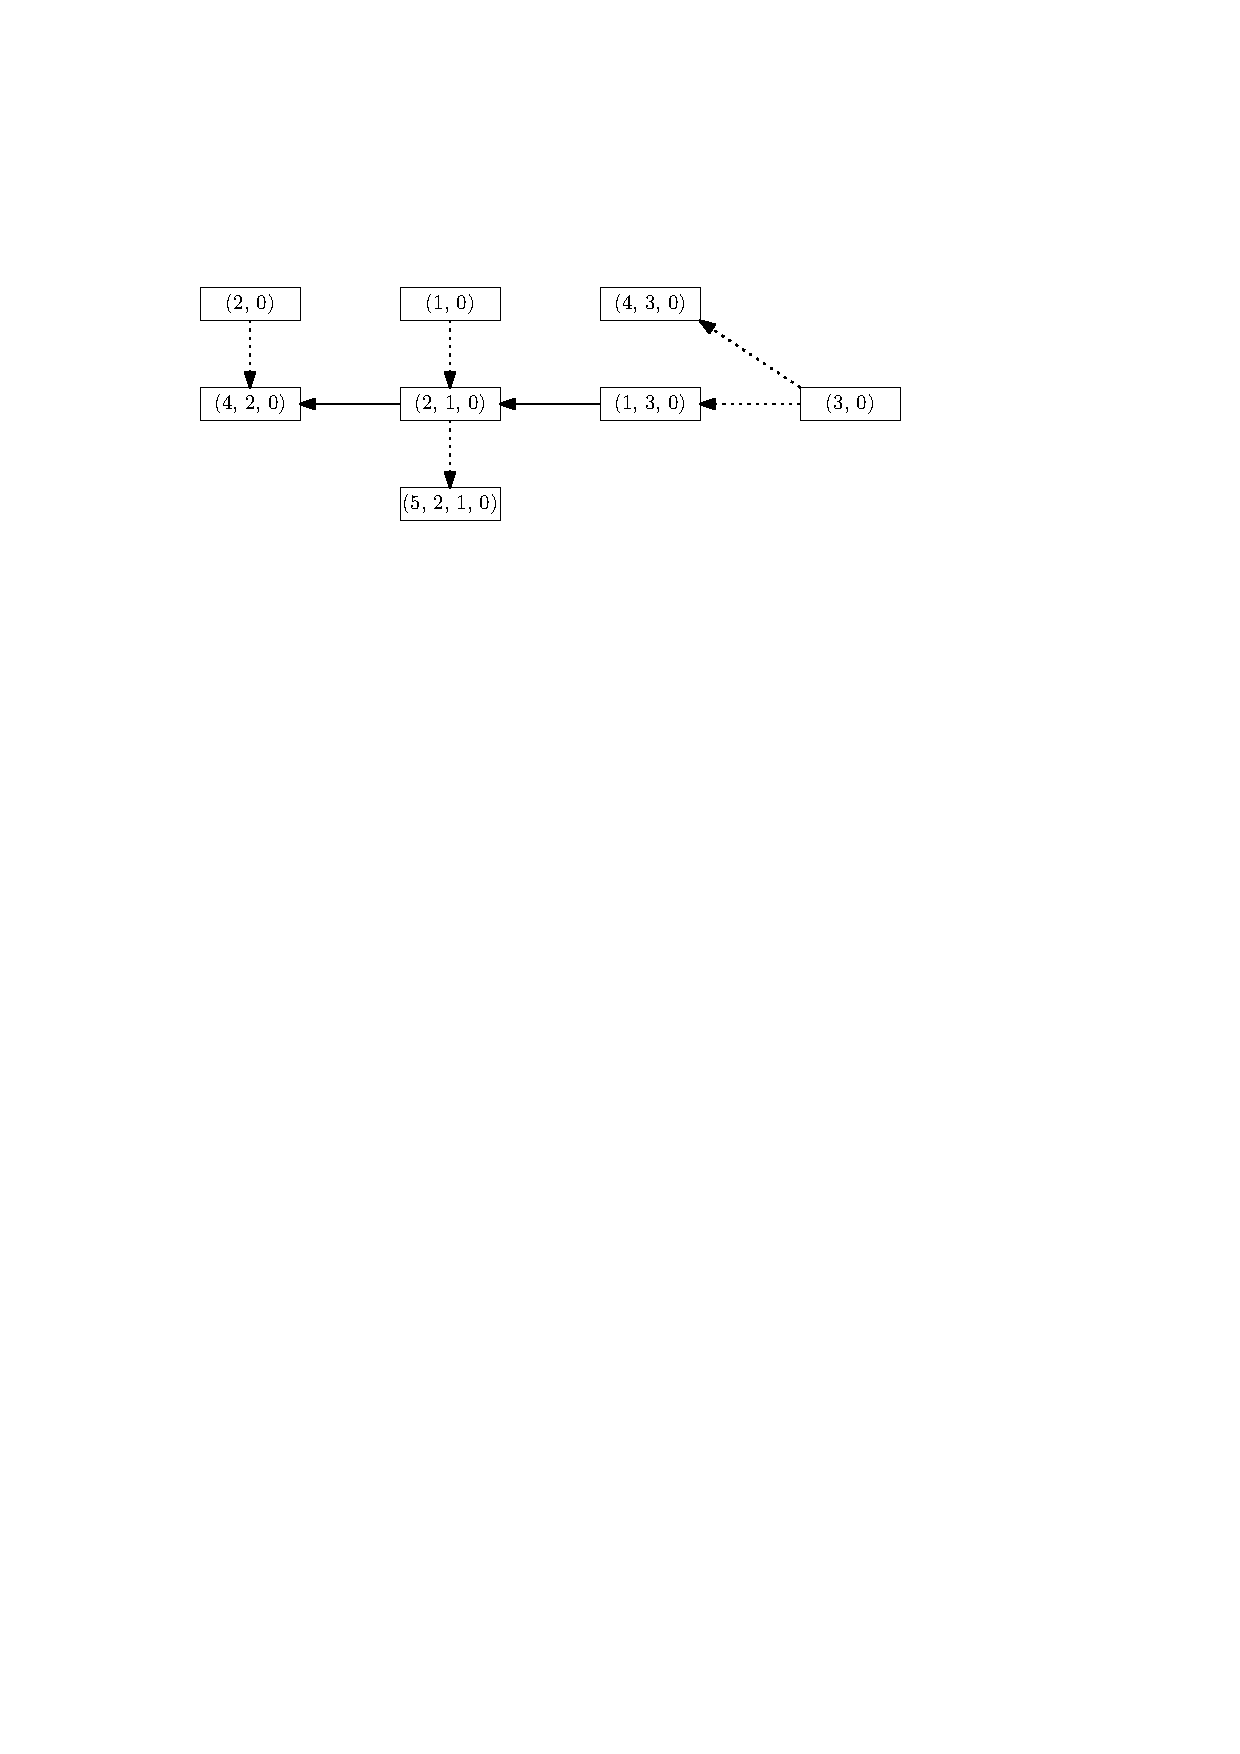
\includegraphics[width=.8\textwidth]{51}
        \end{figure}
    \item The dispute graph for the new system is shown in \cref{52}.
        \begin{figure}[H]
            \centering
            \caption{Dispute Graph for New System}\label{52}
            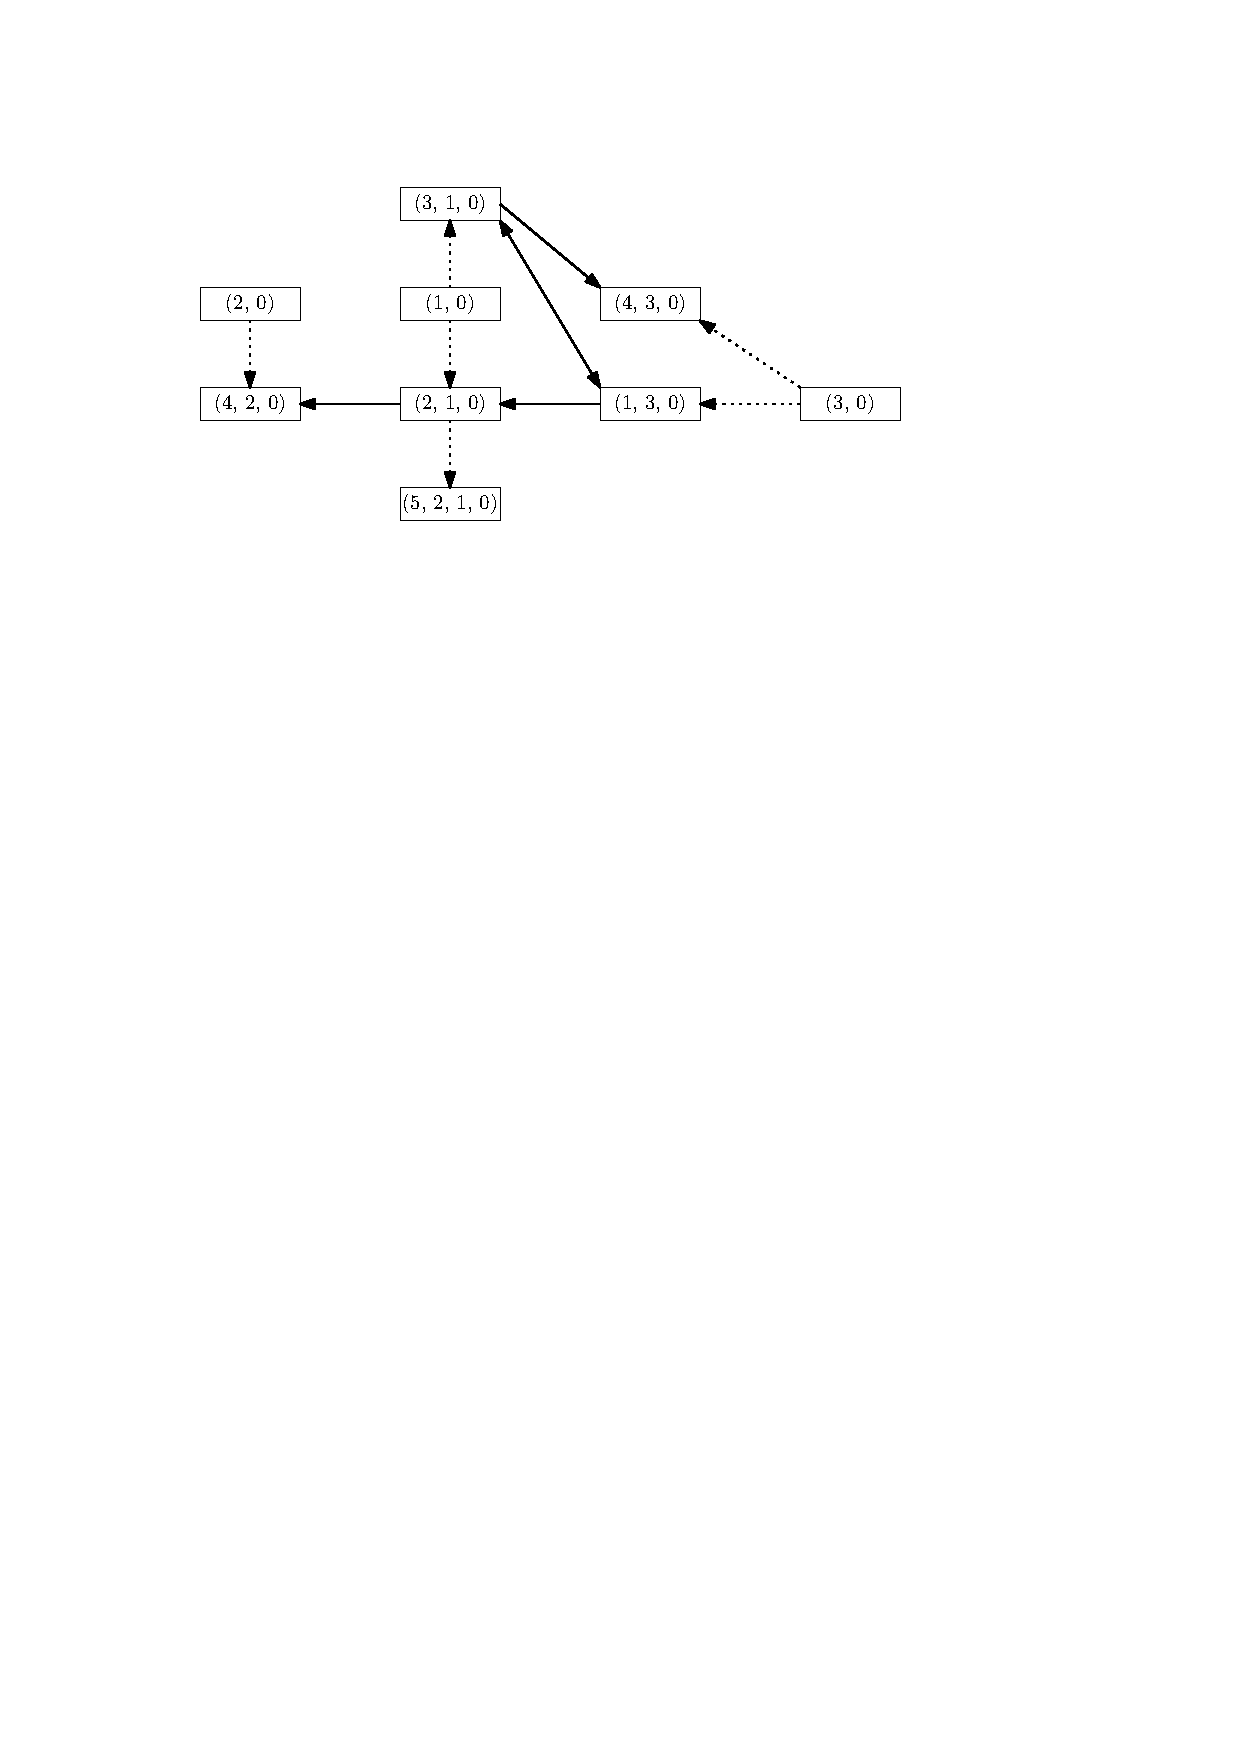
\includegraphics[width=.8\textwidth]{52}
        \end{figure}
    \item
        \begin{enumerate}[label=\roman*. ]
            \item After adding path $[3,1,0]$ to the system, AS0, AS1 and AS3
                became a \textsc{Disagree}.
                Since the rest of the system contains no dispute cycle,
                based on the \textsc{Disagree} we know that
                the system have two stable state as shown in \cref{53}.
                \begin{figure}[H]
                    \centering
                    \caption{Two Stable State of the System}\label{53}
                    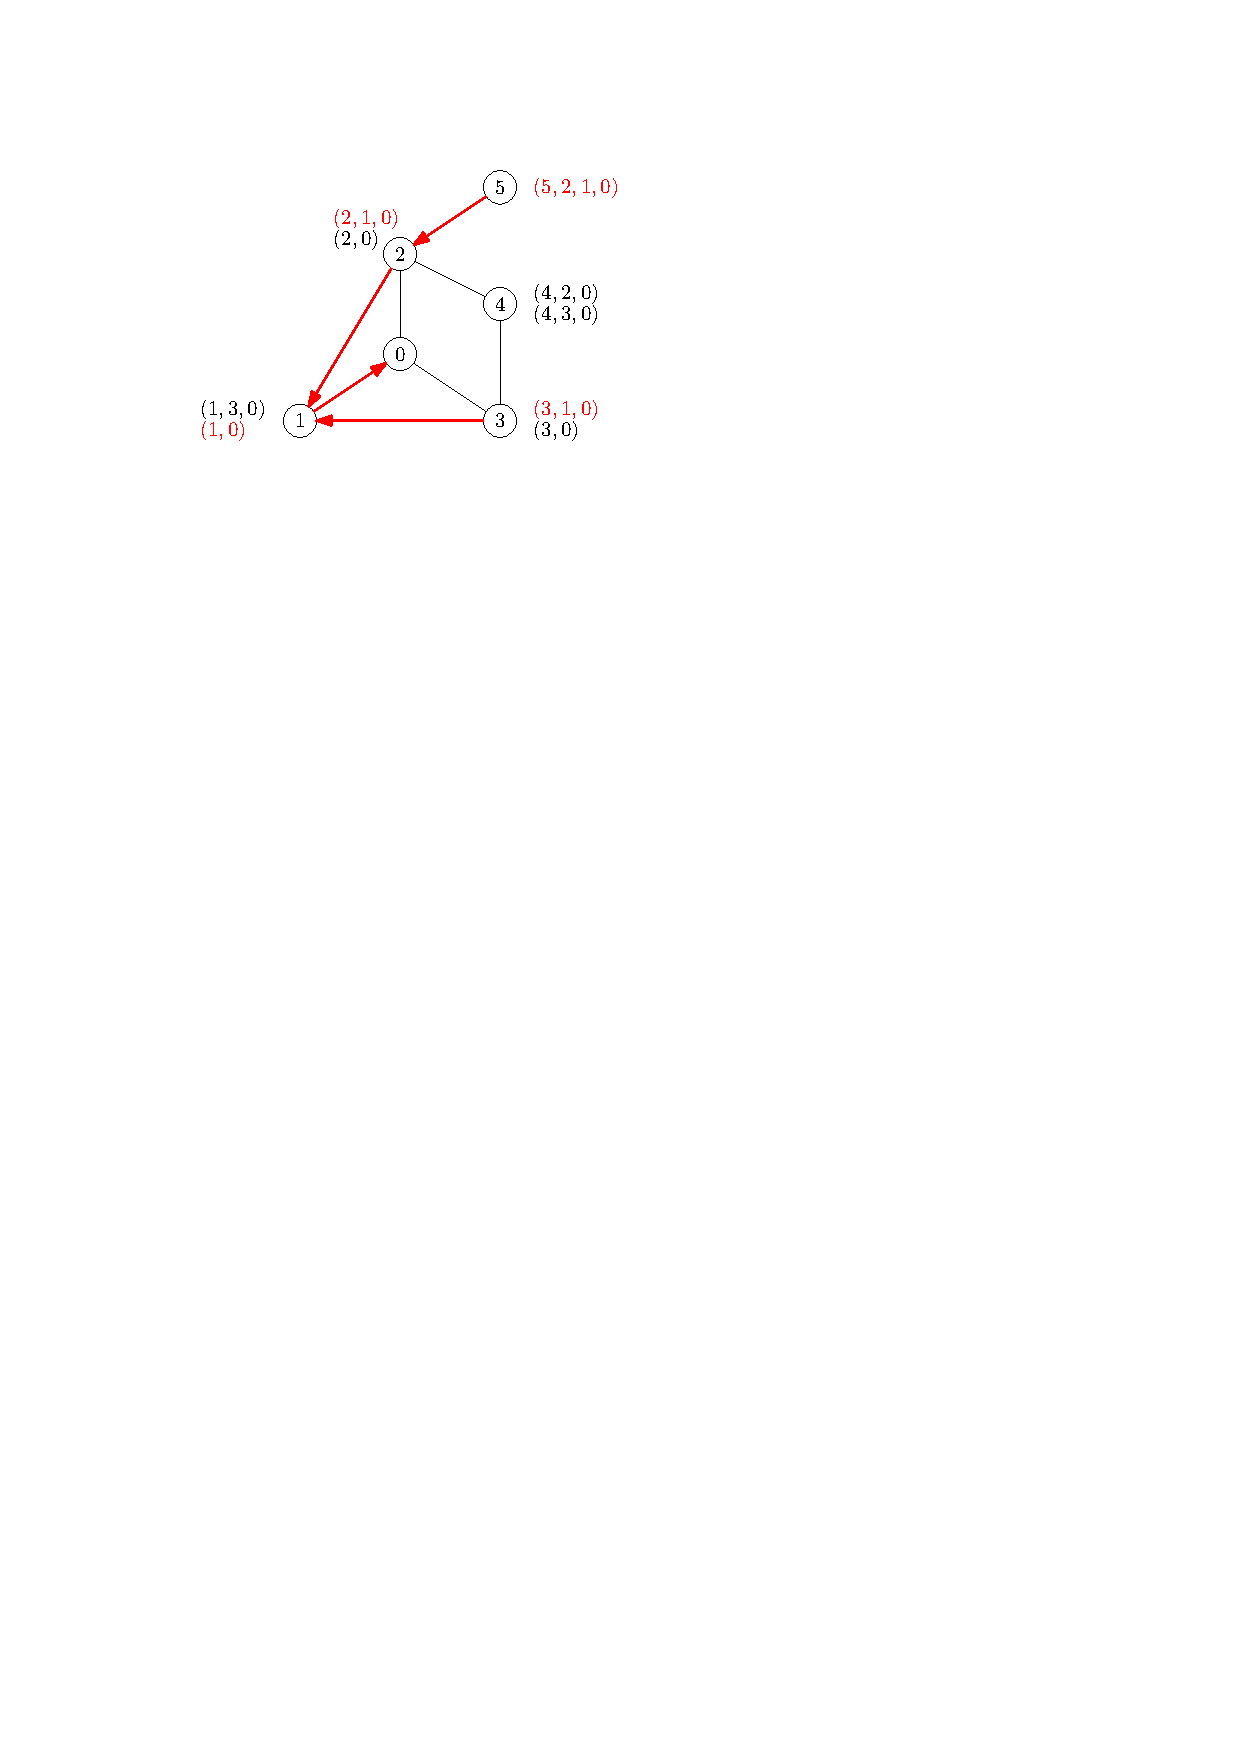
\includegraphics[width=.45\textwidth]{531}
                    \hfill
                    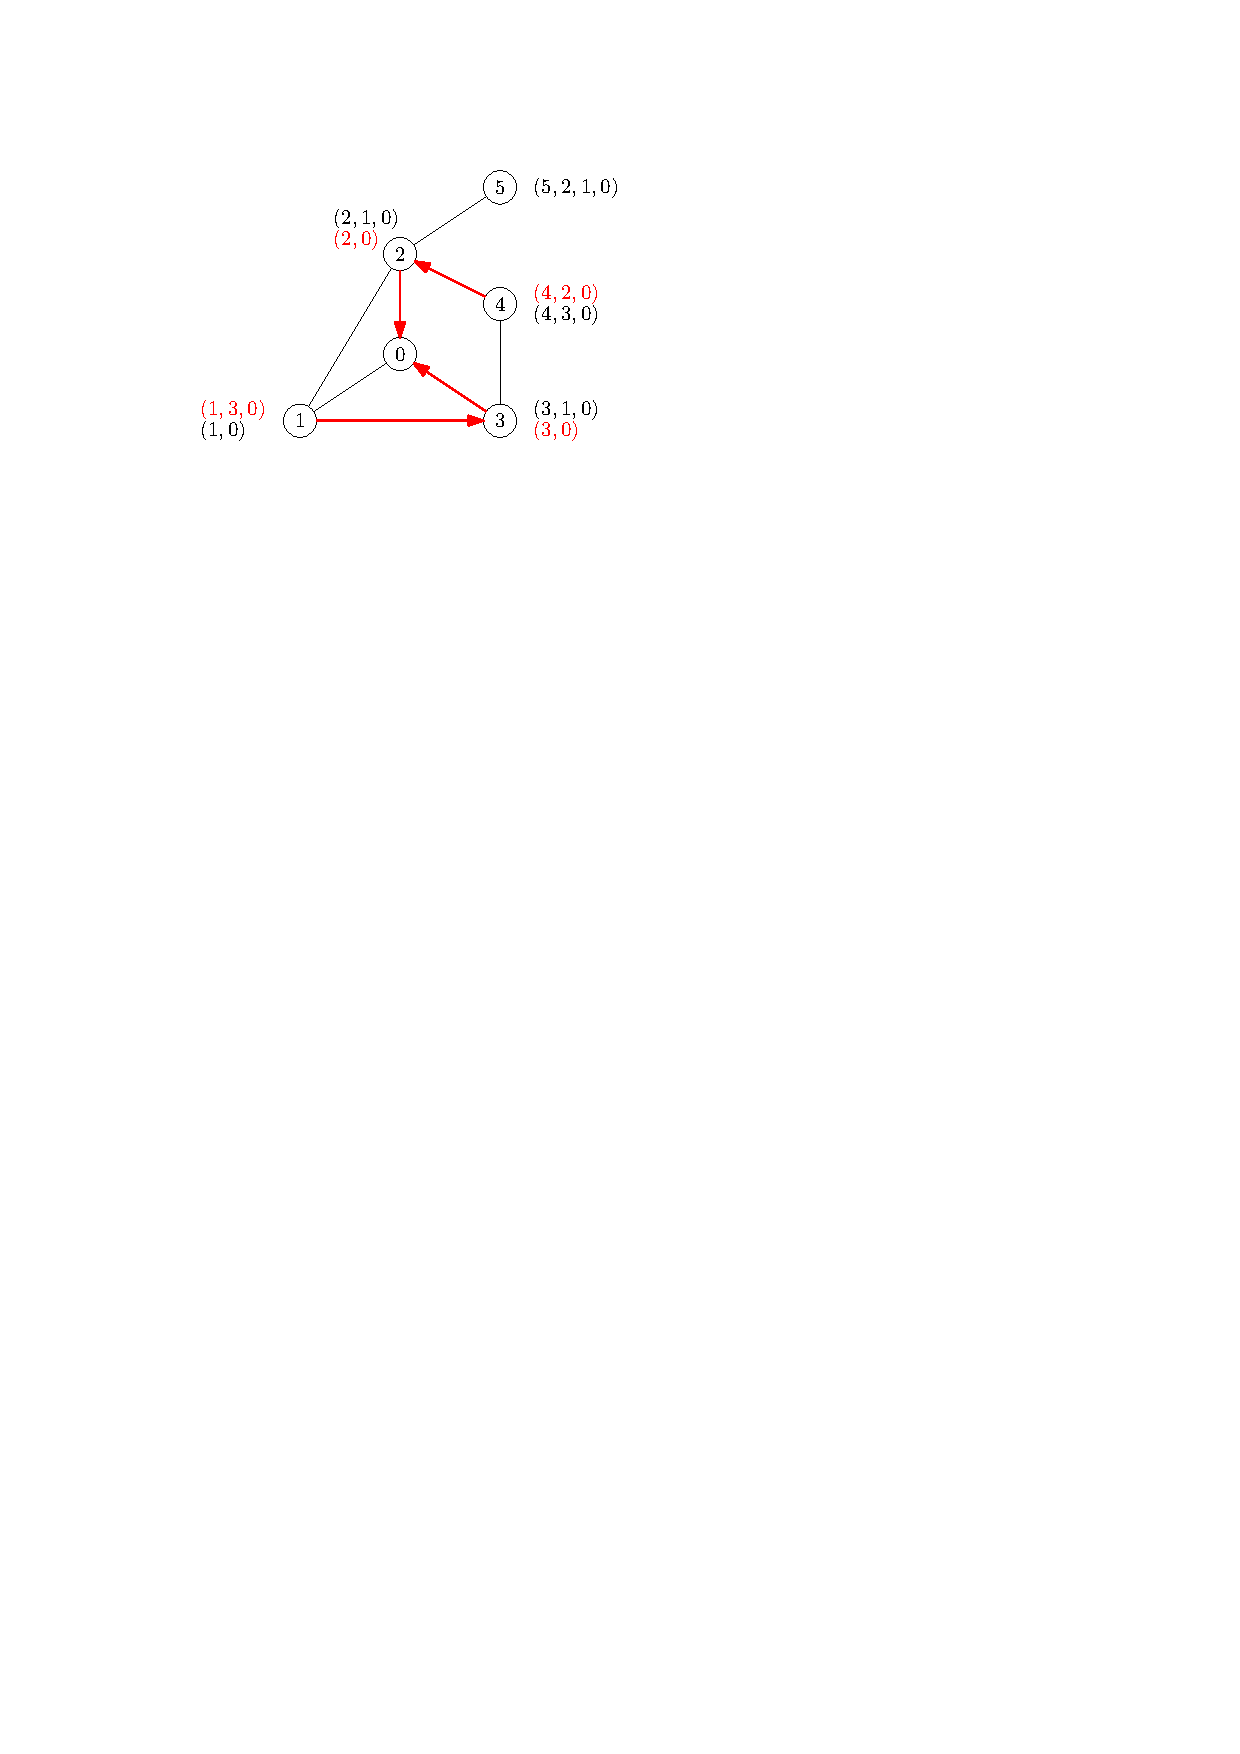
\includegraphics[width=.45\textwidth]{532}
                \end{figure}
            \item The system would always converge.\\
                We know that a \textsc{Disagree} would converge even though it
                contains a dispute cycle(wheel). And the system now has no
                dispute cycle(wheel) other than the \textsc{Disagree}.
                Thus, we can conclude that the system would always converge.
        \end{enumerate}
\end{enumerate}

\section{Hierarchical BGP}
Consider network shown in \cref{6}, with destination \emph{Dst}.
\begin{figure}[H]
    \centering
    \caption{Example}\label{6}
    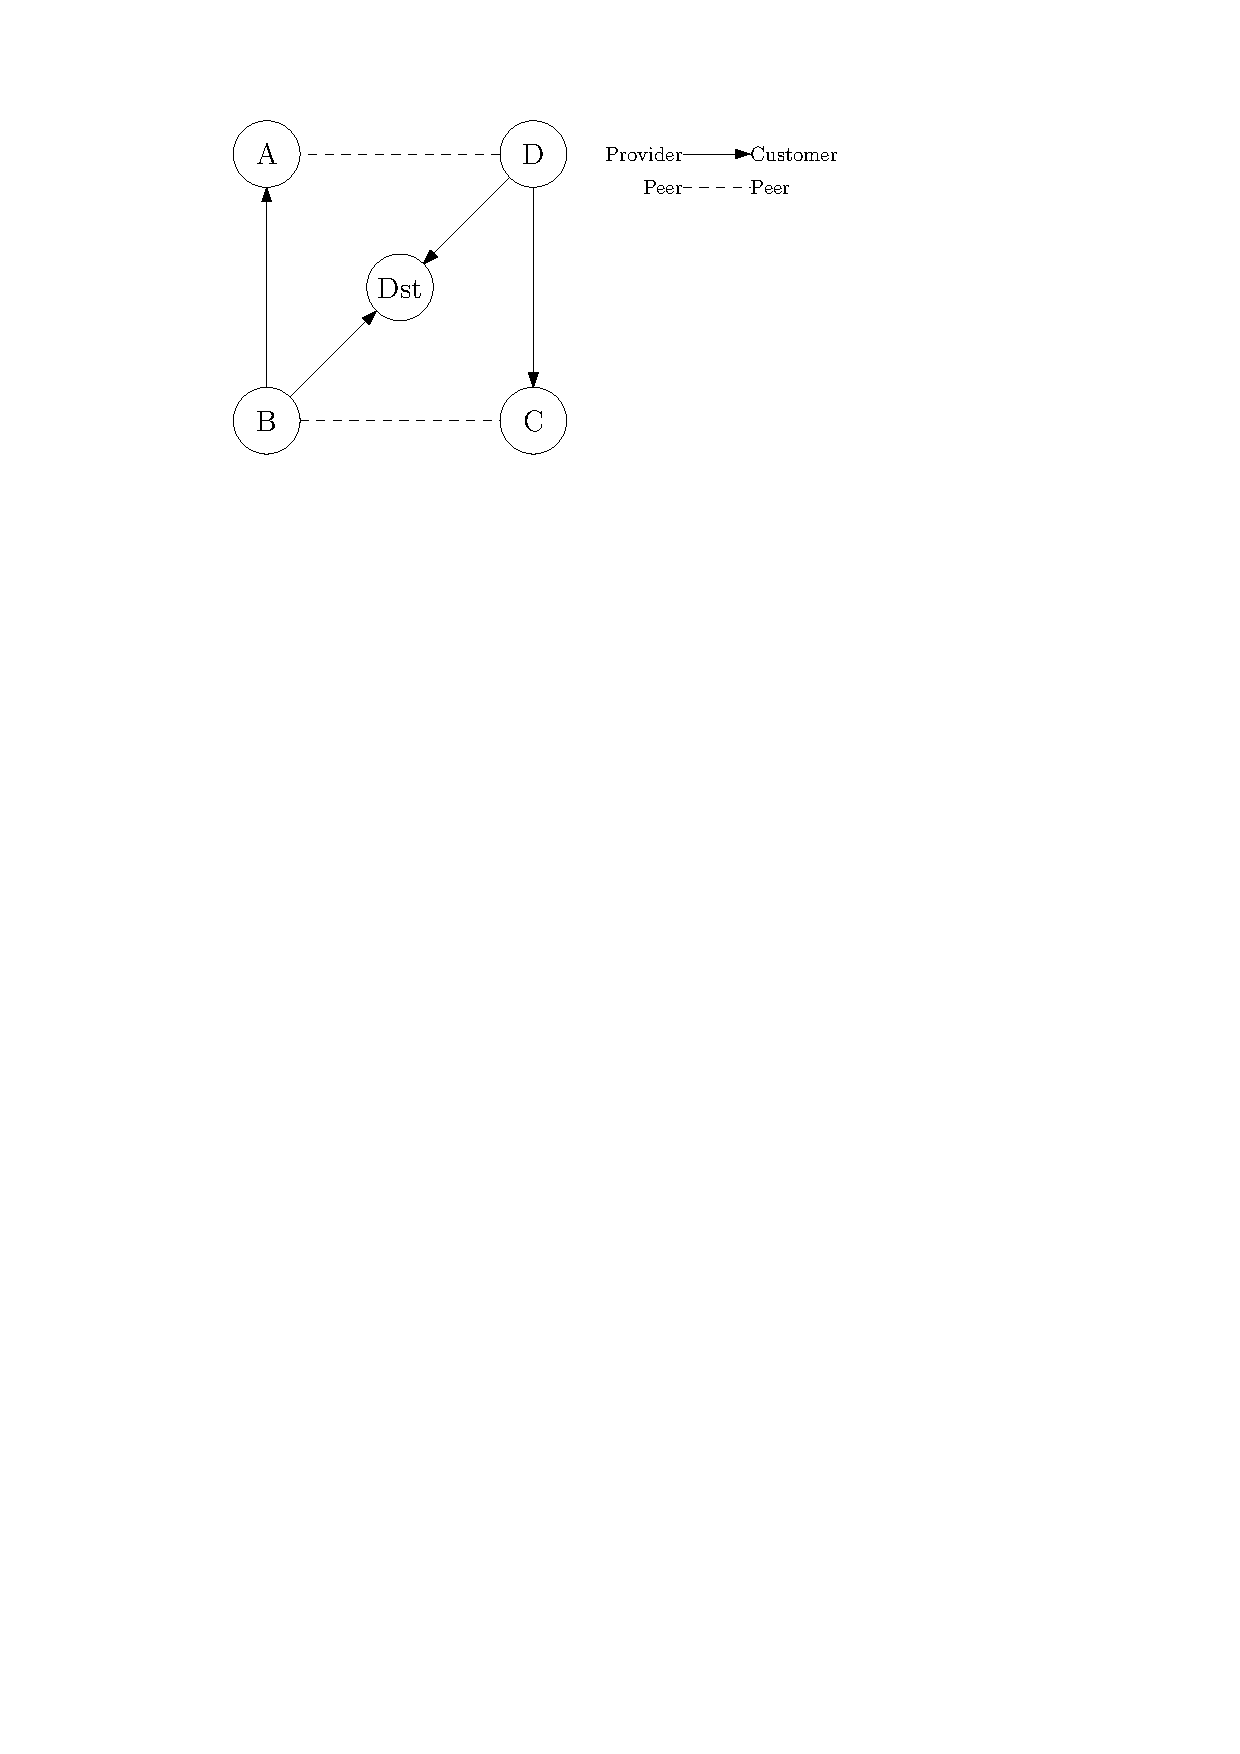
\includegraphics[width=.6\textwidth]{6}
\end{figure}
B is provider to A and Dst, D is provider to C and Dst.
By export policies, B would export its path to Dst to A, and export its path to
A and Dst to C. The same situation falls on D.
Thus, C would learn a path to Dst through B.

Based on local preference, D might prefer C than Dst since both of them are
customers. And C might prefer B than. Since both of them are not customers
of C, C can choose any of them. On the other hand, A might prefer D than B.
In this way, it might result in not acyclic graph and dispute wheel, as shown
in \cref{6d}.
\begin{figure}[H]
    \centering
    \caption{Dispute Wheel Example}\label{6d}
    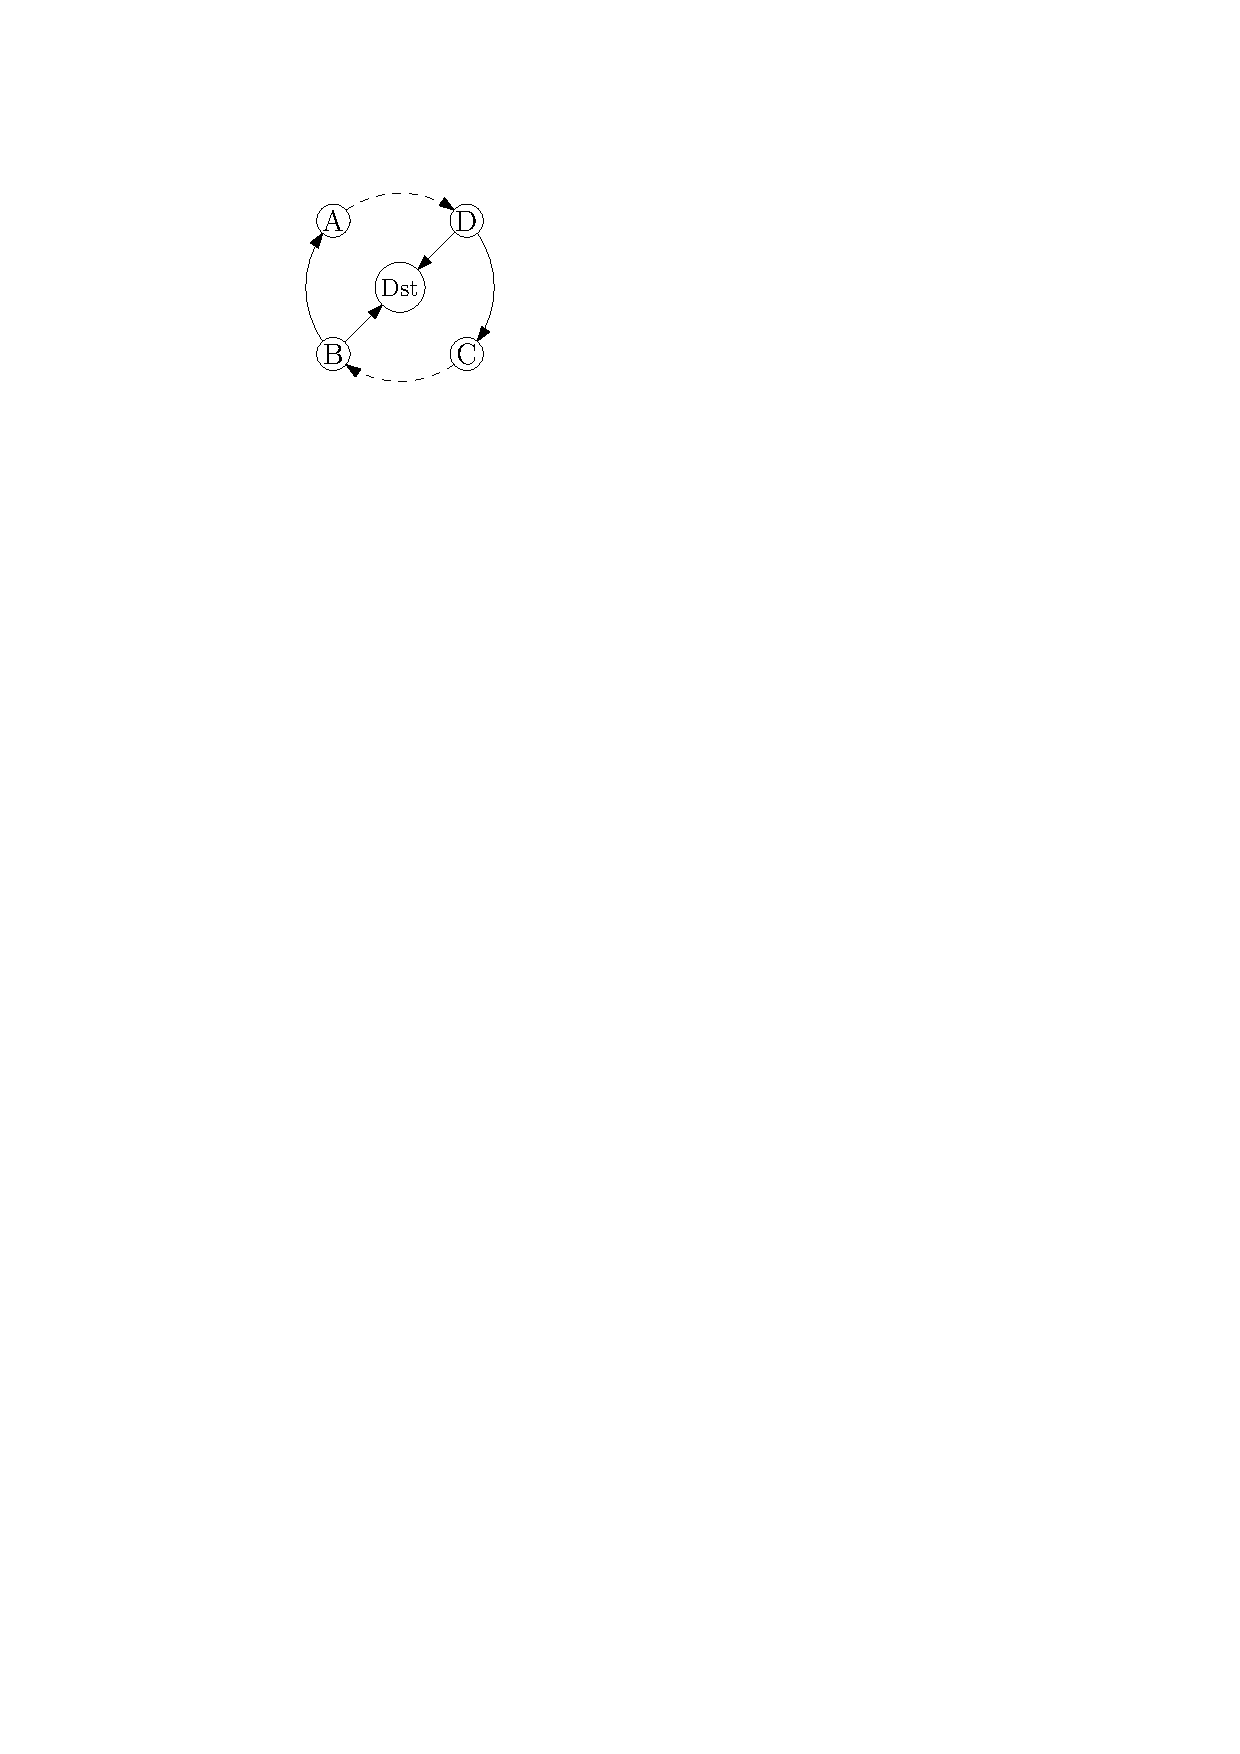
\includegraphics[width=.25\textwidth]{6d}
\end{figure}

\section{Ethernet Multicast}
\begin{enumerate}[label=\bfseries\alph*)]
    \item If the membership reports only flooded some network segments, those
        bridges which does not receive the report will not know whether its
        connected LANs have multicast group members. In this case, if that
        bridge received a multicast message, by default it will not forward it
        to any connected LAN.
    \item It is not possible for Ethernet multicast use flood-and-prune
        approach for several reasons:
        \begin{itemize}[label=-]
            \item Ethernet network segments are connected by bridges, while
                Internet segments are connected by routers. Bridges record the
                outgoing interface for the hosts, while the routers keep a
                routing table including information about next hop and cost.
                A key method used in DVMRP is using the unicast routing table
                to figure out whether the LAN is a child on the tree. Bridges
                can't do that.
            \item Besides, bridge cannot determine whether a connected network
                segment is a `child link' or a `leaf link'. In DVMRP, this is
                achieved via \emph{split horizon with poisoned reverse}.
                However, bridges in Ethernet do not exchange routing
                informations.
        \end{itemize}
\end{enumerate}

\section{Reverse Path Flooding}

\begin{enumerate}[label=\bfseries\alph*)]
    \item In distance vector routing, routers will exchange each other's
        distance vector. So a router would know its neighbor's distance to the
        source. If neighbor's distance to source is smaller than the router's
        distance plus the cost between them two, there is apparently no need to
        send the broadcast messages to that neighbor, because the neighbor must
        have a shorter path to get the that broadcast message.\\
        In this way, each router would receive the broadcast message only once.
    \item In link-state routing, each router could compute the shortest path to
        every LANs. Thus the router only need to send broadcast message to
        those paths and routers along that path would forward the message to
        the rest of the network through their computed shortest paths.
        Apparently, if the shortest path to some LANs is through the incoming
        interface, that LAN don't need current router to forward the broadcast
        message.\\
        In this way, each router would receive the broadcast message only once.
\end{enumerate}

\section{DVMRP}
\begin{enumerate}[label=\bfseries\roman*.]
    \item The path of broadcast is shown in \cref{91}. Parent router for each
        LAN is marked in the figure.
        \begin{figure}[H]
            \centering
            \caption{Path of Broadcast Messages}\label{91}
            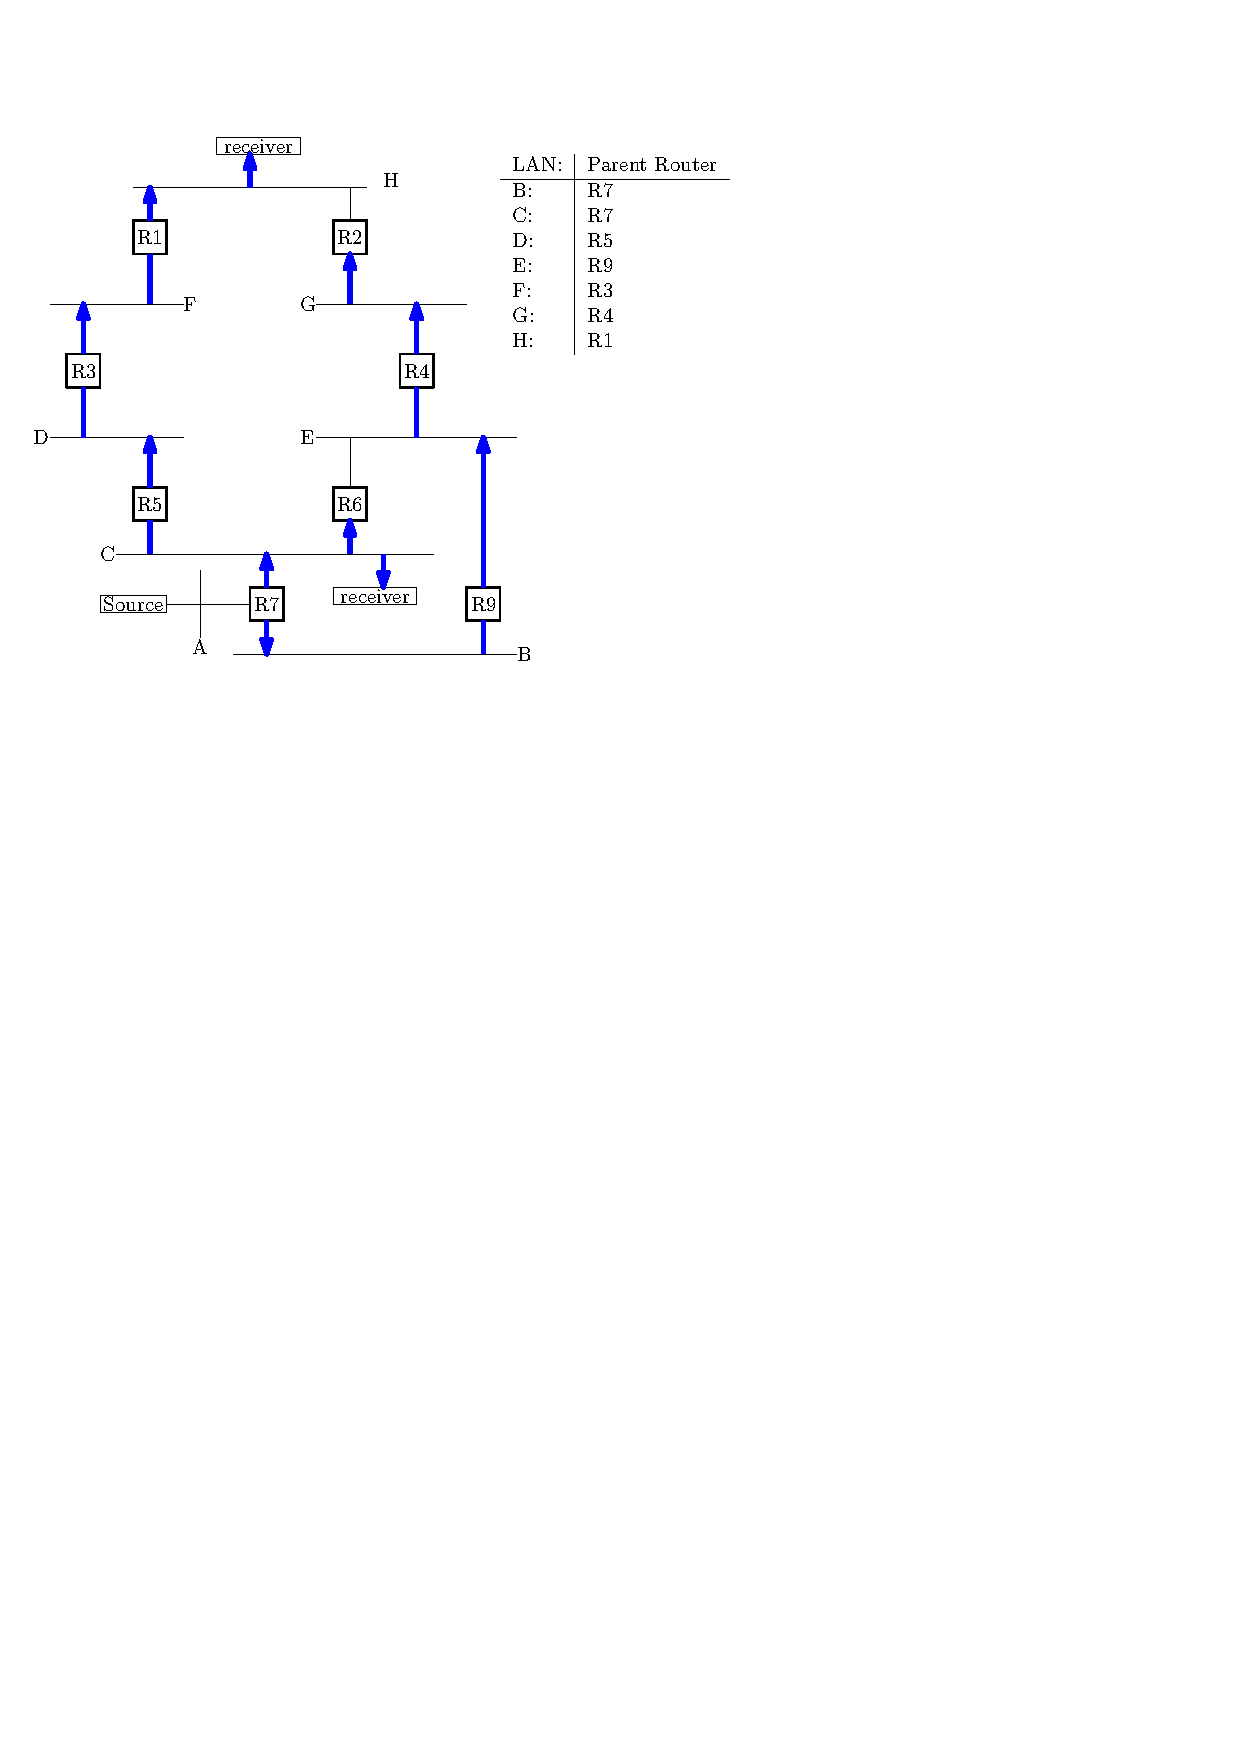
\includegraphics[width=.9\textwidth]{91}
        \end{figure}
    \item In Truncated Reverse Path Broadcast, only LAN G is a leaf LAN.
        Because R2 does not need to send broadcast message to LAN H, and LAN G
        itself does not have a group member host.\pagebreak
    \item Non-Membership Reports are shown in red dashed line in \cref{93}.
        \begin{figure}[H]
            \centering
            \caption{Non-Membership Reports}\label{93}
            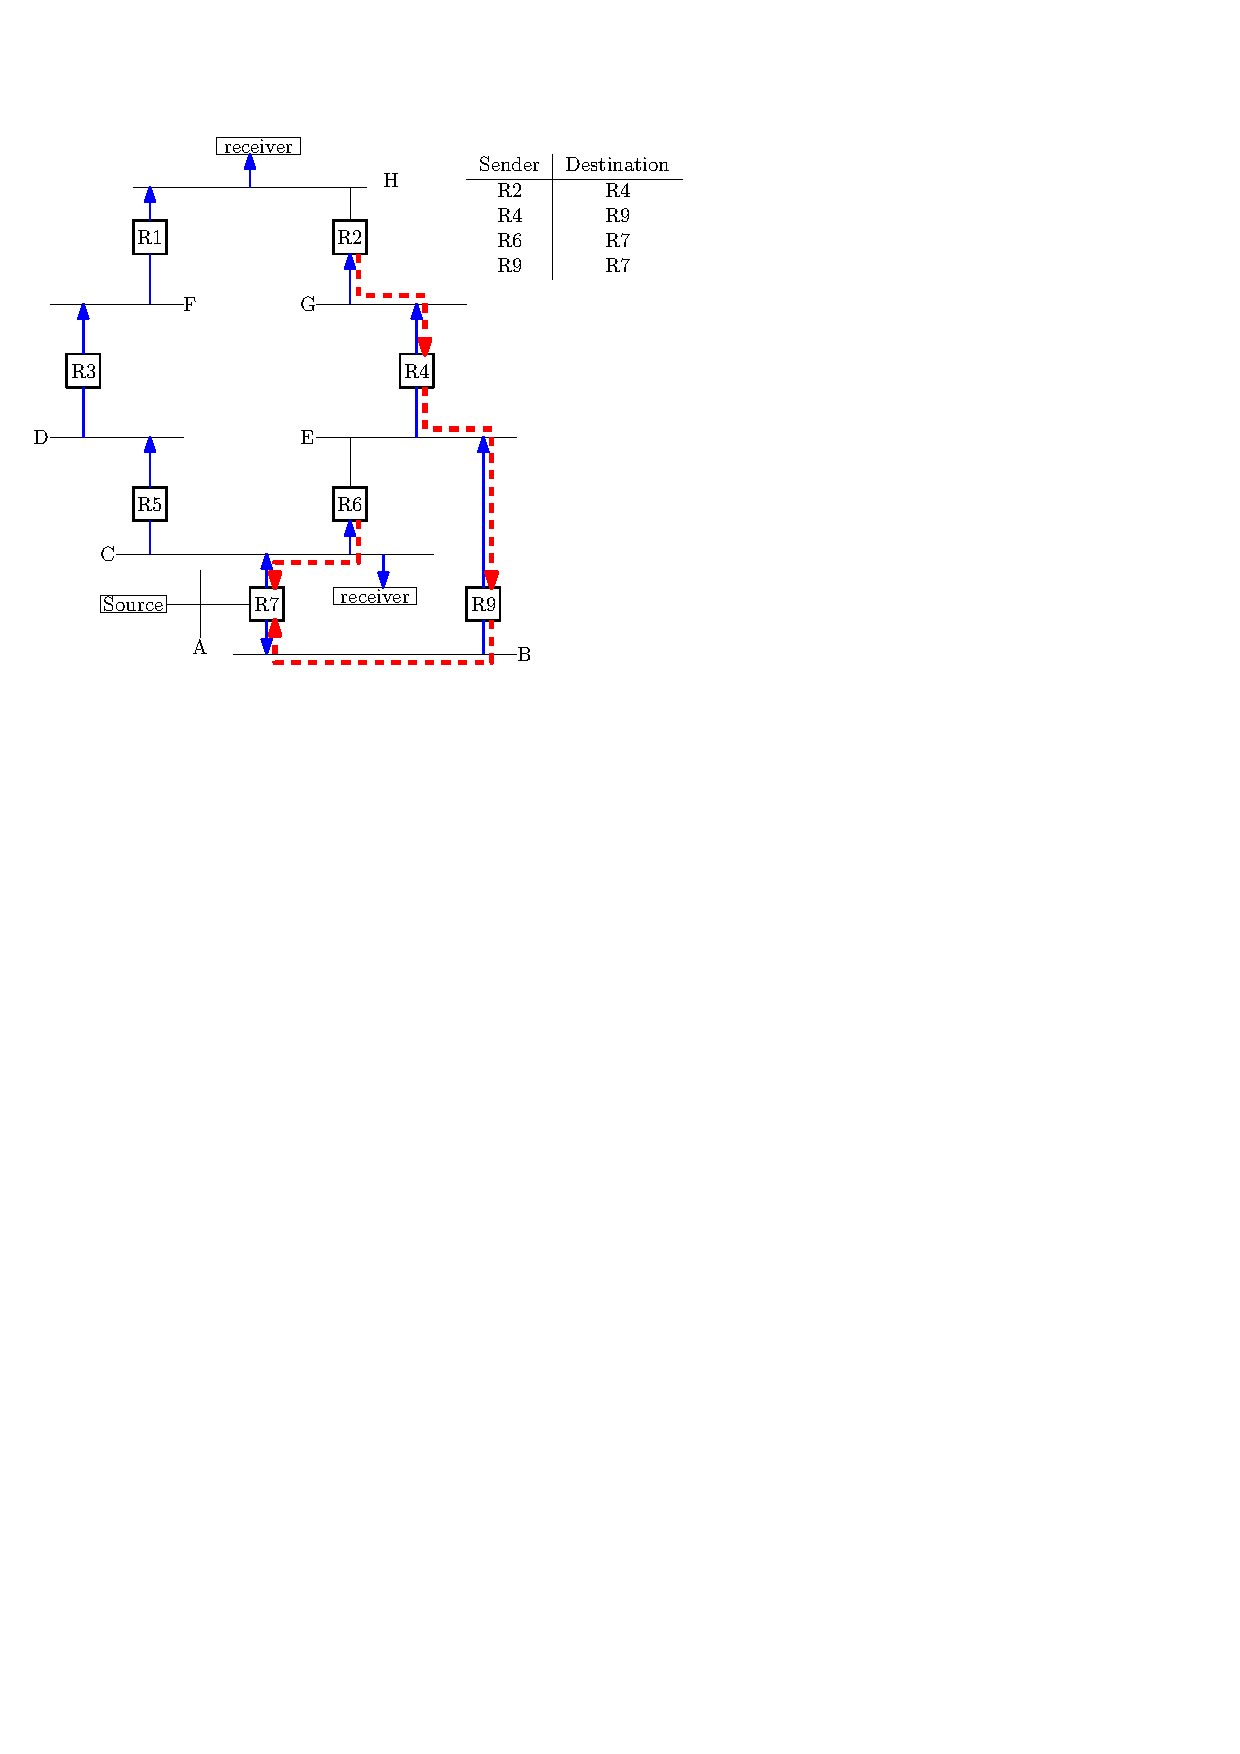
\includegraphics[width=.65\textwidth]{93}
        \end{figure}
    \item After pruning, LANs over which multicast messages from S are sent to
        are: \texttt{C D E H}, as shown in \cref{94}.
        \begin{figure}[H]
            \centering
            \caption{After Pruning Message Flow}\label{94}
            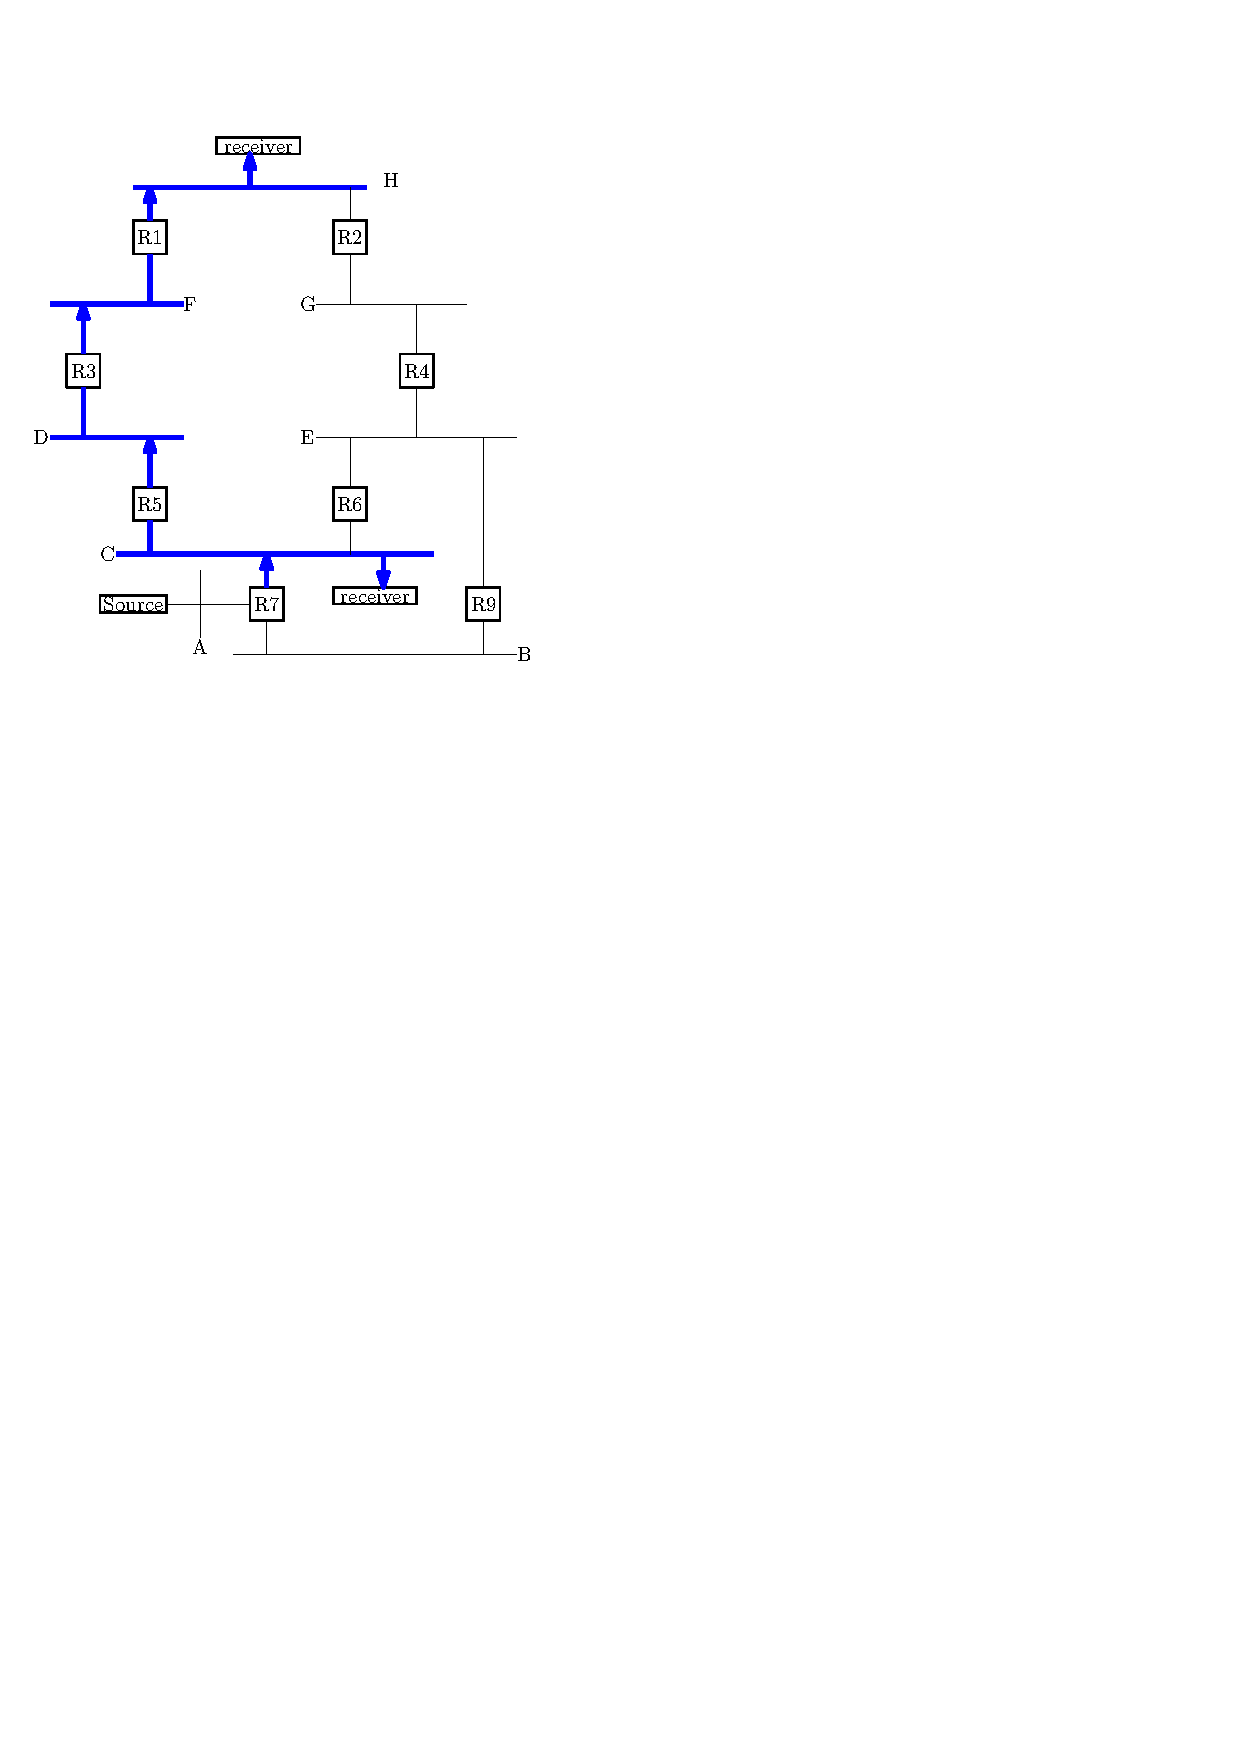
\includegraphics[width=.521\textwidth]{94}
        \end{figure}
\end{enumerate}

\end{document}
